%%%%%%%%%%%%%%%%%%%%%%%%%%%%%%%%%%%%%%%%%
% Tutorial
% LaTeX Template
% Version 1.0 (05/11/17)
%
% Author:
% Ben Roose (ben.roose@wichita.edu)
%
% Original template author:
% Adam Glesser (adamglesser@gmail.com)
% www.LaTeXTemplates.com
%
% License:
% CC BY-NC-SA 3.0 (http://creativecommons.org/licenses/by-nc-sa/3.0/)
%
%%%%%%%%%%%%%%%%%%%%%%%%%%%%%%%%%%%%%%%%%

\documentclass[12pt]{article}

\usepackage{graphicx} %Allow import of images
\graphicspath{ {images/} } % Relative path to images directory
\usepackage[margin=1in]{geometry} % Required to make the margins smaller to fit more content on each page
\usepackage[linkcolor=blue]{hyperref} % Required to create hyperlinks to questions from elsewhere in the document
\hypersetup{pdfborder={0 0 0}, colorlinks=true, urlcolor=blue} % Specify a color for hyperlinks
\usepackage{todonotes} % Required for the boxes that questions appear in
\usepackage{tocloft} % Required to give customize the table of contents to display questions
\usepackage{microtype} % Slightly tweak font spacing for aesthetics
\usepackage{palatino} % Use the Palatino font

\setlength\parindent{0pt} % Removes all indentation from paragraphs

% Create and define the list of questions
\newlistof{questions}{faq}{\large FAQ for accessing the Routing \& Switching Lab in EE 328C and 328D} % This creates a new table of contents-like environment that will output a file with extension .faq
\setlength\cftbeforefaqtitleskip{3em} % Adjusts the vertical space between the title and subtitle
\setlength\cftafterfaqtitleskip{1em} % Adjusts the vertical space between the subtitle and the first question
\setlength\cftparskip{.3em} % Adjusts the vertical space between questions in the list of questions

% Create the command used for questions
\newcommand{\question}[1] % This is what you will use to create a new question
{
\refstepcounter{questions} % Increases the questions counter, this can be referenced anywhere with \thequestions
\par\noindent % Creates a new unindented paragraph
\phantomsection % Needed for hyperref compatibility with the \addcontensline command
\addcontentsline{faq}{questions}{#1} % Adds the question to the list of questions
\todo[inline, color=green!40]{\textbf{#1}} % Uses the todonotes package to create a fancy box to put the question
\vspace{1em} % White space after the question before the start of the answer
}

% Uncomment the line below to get rid of the trailing dots in the table of contents
%\renewcommand{\cftdot}{}

% Uncomment the two lines below to get rid of the numbers in the table of contents
%\let\Contentsline\contentsline
%\renewcommand\contentsline[3]{\Contentsline{#1}{#2}{}}

\begin{document}

%----------------------------------------------------------------------------------------
%	TITLE AND LIST OF QUESTIONS
%----------------------------------------------------------------------------------------

\begin{center}
\Huge{\bf \emph{EECS Tutorial: Routing \& Switching Lab}} % Main title
\end{center}

\listofquestions % This prints the subtitle and a list of all of your questions
\bigskip % Create a gap between list and first question

%\newpage % Comment this if you would like your questions and answers to start immediately after table of questions

%----------------------------------------------------------------------------------------
%	QUESTIONS AND ANSWERS
%----------------------------------------------------------------------------------------

\question{What is the default login username and password for Arista switches?}\label{password}

\begin{verbatim}
Username: student
Password: arista
\end{verbatim}

%------------------------------------------------

\question{How do I access rslab equipment from a mobile Linux terminal in EE 328C?}\label{mobile_terminals}

\begin{enumerate}
\item In EE 327C turn on a mobile Linux terminal. Computer will network boot from the rslab LTSP server and automatically log into a GUI desktop environment.
\item Open \textit{PAC Manager} from the Desktop or the \textit{applications} menu.
\item On left side, double-click the terminal server for the rack \# assigned to you by GTA. A new session tab window will open and connect into the terminal server.
\item Once connected to the terminal server for your assigned rack, use the menu options to connect into and disconnect from the Arista switches and Cisco router in the EE 328D networking rack.
\item At any time you can return to the terminal server menu by pressing \texttt{CTRL+SHIFT+7}.
\item To view all open connections in the session, return to the menu and press \texttt{16}.
\item To exit from the terminal server, return to the menu and press \texttt{18}.
\end{enumerate}

\textbf{NOTE:} You can open more than one tabbed session within \textit{PAC Manager} to access the same rack terminal server and connect to multiple network devices concurrently, but each switch or router can only be accessed by one terminal server session at a time.

\begin{figure}[h]
\caption{Example of connecting with \textit{PAC Manager} from a mobile Linux terminal}
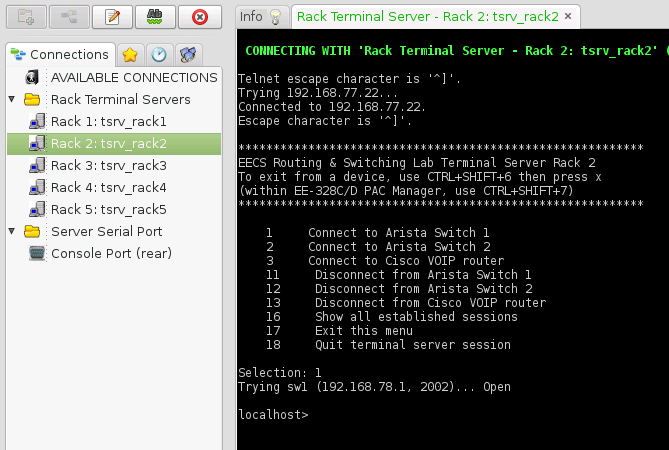
\includegraphics[width=\linewidth]{screenshot_pac}
\centering
\end{figure}

\newpage
%------------------------------------------------

\question{How do I access rslab equipment from a computer outside of EE 328C?}\label{remote_access}

\begin{enumerate}
\item Due to WSU security, rslab devices can only be accessed via an EECS Linux server.
\item Follow \textit{Remote Access EECS Linux Servers.pdf} first to log into an EECS Linux Server.
\item Once logged into an EECS Linux server, use SSH to access the rslab proxy server, by typing into a shell window (where \texttt{\#} is the rack number assigned to you by GTA):
\begin{verbatim}
ssh -t rslab telnet rack#
\end{verbatim}

\item Enter your myWSU password when prompted to do so.
\item You may see a "\texttt{Could not chdir...}" error message when you open a connection to the rslab proxy server. Disregard this message. The proxy server does not need access to your user home directory for access to the rslab terminal servers in EE 328D.
\item Once connected to the terminal server for your assigned rack, use the menu options to connect into and disconnect from the Arista switches and Cisco router in the EE 328D networking rack.
\item At any time you can return to the terminal server menu by pressing \texttt{CTRL+SHIFT+6} and then \texttt{x}.
\item To view all open connections in the session, return to the menu and press \texttt{16}.
\item To exit from the terminal server and close the remote SSH connection to the rslab proxy server, return to the menu and press \texttt{18}.
\end{enumerate}
\textbf{NOTE:} You can open multiple command-line/shell windows from your client machine to access the same rack terminal server and connect to multiple network devices concurrently, but each switch or router can only be accessed by one terminal server session at a time. You can also use a terminal multiplexer such as \textit{tmux} or \textit{screen} within any of the EECS Linux servers to open multiple, simulaneous SSH sessions to an rslab terminal server.

\begin{figure}[h]
\caption{Example of SSH remote connection via rslab proxy server}
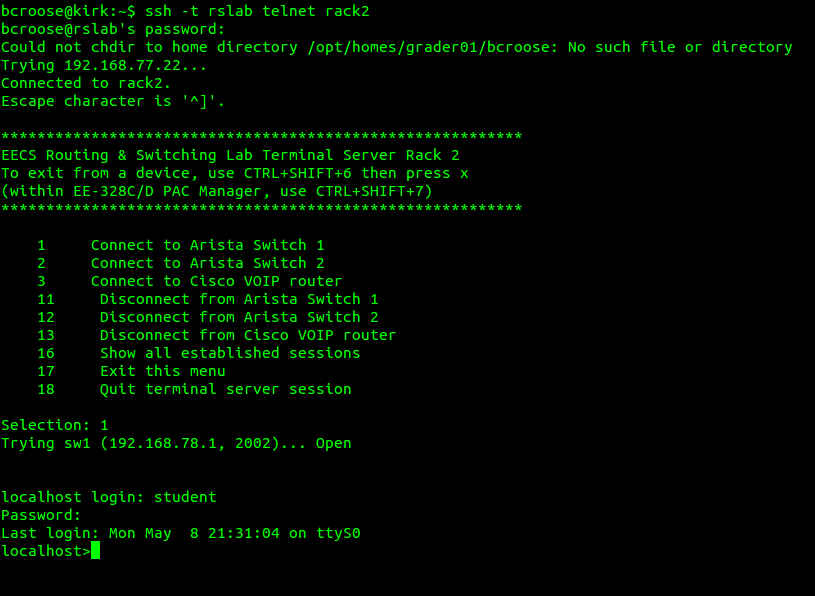
\includegraphics[width=\linewidth]{screenshot_ssh}
\centering
\end{figure}

\newpage
%------------------------------------------------

\question{Why do I sometimes see "\texttt{\% Connection refused by remote host}"? }\label{connection_refused}

Though you can open multiple connection sessions to the terminal server controlling each rack, you can only access each network switch or router device within the rack from a single terminal server session.\\\\
This access restriction is caused by limitations of the serial communication protocol between the terminal server and each network device in the rack. The access restriction also acts as a security failsafe, since it reduces the possibility of more than one person or lab group attempting to make changes to a switch or router configuration concurrently.\\

If you see the "\texttt{\% Connection refused by remote host}" error, then either you already have opened a connection to this network device in another terminal server session or another person/lab group has an open connection to this network device. Check you do not already have an open connection in another terminal server session first, then speak with the lab GTA if you cannot resolve the connection refused error yourself.\\


%------------------------------------------------

\question{How do I create a screenshot of my lab session?}\label{screenshot}

\subsection*{EE 328C Linux Terminals}
Within the EE 328C mobile Linux terminals there are three screenshot tools: pressing \texttt{Print Screen} key, using \textit{Take Screenshot} located on the Desktop, or using \textit{PAC Manager's} \textbf{Take Screenshot} menu option.

\subsection*{Remote Access Clients}
Most Windows, Linux and Mac client systems have screenshot tools, which can be used to screenshot the remote access terminal window. Please see your system's documentation for further help.

\newpage
%------------------------------------------------

\question{How do I create a text log of my entire lab session?}\label{logging}

\subsection*{EE 328C Linux Terminals}
Within the EE 328C Linux terminals, \textit{PAC Manager} can log all session data to a text file.
\begin{enumerate}
\item Right-click on the session title tab and select \textbf{Save session log...} from the menu.
\item Enter a name for the log file and click \textbf{Enter} button to save.
\end{enumerate}

\subsection*{Remote Access Clients: Linux}
When accessing the rslab remotely from a Linux terminal window, a session log can be specified at the start of the remote SSH session by typing into a terminal window: 
\begin{verbatim}
ssh -t rslab telnet rack# | tee log_filename
\end{verbatim}

where \texttt{\#} is the rack number assigned to you by GTA and log\_filename is the path and filename for the log, i.e.
\begin{verbatim}
ssh -t rslab telnet rack2 | tee cs764_lab/assignment1_log.txt
\end{verbatim}

\subsection*{Remote Access Clients: Windows}
When accessing the rslab remotely with PuTTY on a Windows client, a session log can be specified at the start of the remote SSH session by configuring PuTTY's logging function:
\begin{enumerate}
\item In the \textit{PuTTY Configuration} window, click on \textbf{Logging} category on the left.
\item Select \textbf{All session output} and click on \textbf{Browse} button.
\item Enter a name for the log file and click \textbf{Save} button to save.
\item \textit{Optional:} Logging options can be saved as part of a host connection session in the \textit{PuTTY} \textbf{Saved Sessions} list.
\item For further help on configuring logging in \textit{PuTTY}, see:\\ 
\href{http://www.tricksguide.com/guide-how-to-capture-a-log-file-of-your-putty-session.html}{SiRu's guide on tricksguide.com}
\end{enumerate}


%----------------------------------------------------------------------------------------

\end{document}